
%(BEGIN_QUESTION)
% Copyright 2010, Tony R. Kuphaldt, released under the Creative Commons Attribution License (v 1.0)
% This means you may do almost anything with this work of mine, so long as you give me proper credit

En forsker bygger en eksperimentell solfanger for varmluft med en sløyferegulator for å holde konstant innetemperatur uavhengig av solinnstråling:

$$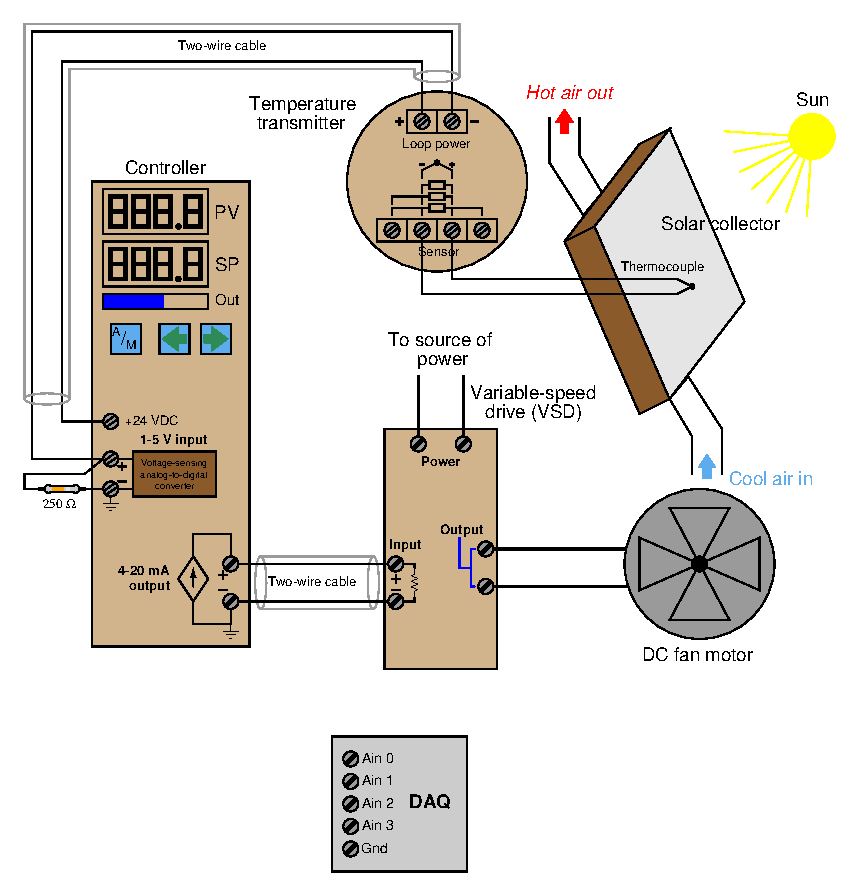
\includegraphics[width=15.5cm]{i01417x01.eps}$$

Forskeren ønsker også å logge temperatur- og viftekommandosignalene (PV og Output) med en datainnsamlingsmodul (DAQ) koblet til en PC. DAQ-en kan måle DC-spenningssignaler fra 0 til +7.5 volt (single-ended), omtrent som et firekanals DC-voltmeter med felles negativ terminal.

\vskip 10pt

Skisser nødvendige tilkoblingsledninger for at denne DAQ-enheten skal kunne måle temperatursignalet på inngang Ain2 og viftekommandosignalet på inngang Ain0.

\vfil 

\underbar{file i01417}
\eject
%(END_QUESTION)





%(BEGIN_ANSWER)

Dette er et gradert spørsmål -- ingen svar eller hint gis!
 
%(END_ANSWER)





%(BEGIN_NOTES)

At DAQ-en har én felles negativ terminal for alle fire innganger, kombinert med at både regulatorens PV-inngang og utgang deler felles jord, gjør det mulig å måle disse to datapunktene med bare tre ledninger mellom regulator og DAQ:

$$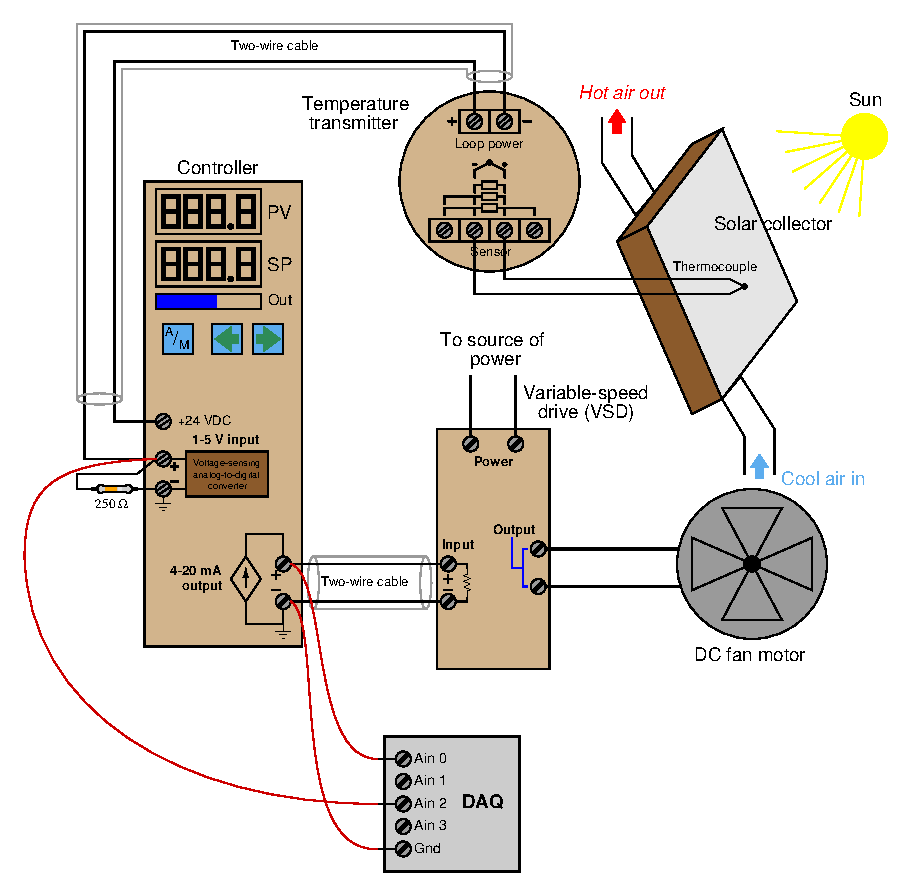
\includegraphics[width=15.5cm]{i01417x02.eps}$$

Alternativt kan ``Gnd''-terminalen på DAQ kobles til ($-$)-terminalen på PV-inngangen i stedet for ($-$)-terminalen på regulatorens utgang.

%INDEX% Pictorial circuit review (analog signal wiring to data acquisition unit)

%(END_NOTES)

